\documentclass{standalone}
\usepackage{tikz}
\usetikzlibrary{shapes.geometric, arrows}

\tikzstyle{block} = [rectangle, draw, fill=blue!20,
    text centered, minimum height=3em, minimum width=6em]
\tikzstyle{line} = [draw, -latex']

\begin{document}
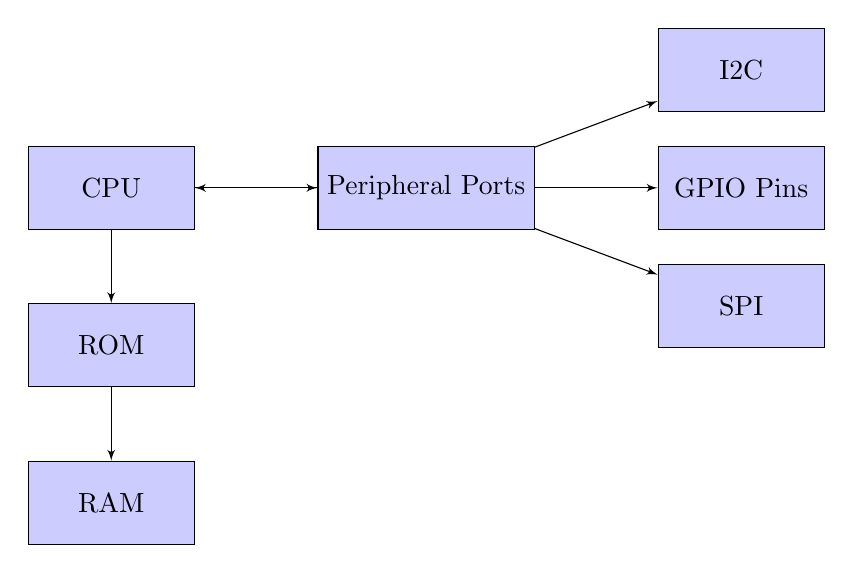
\begin{tikzpicture}[node distance=2cm, auto]

    \node [block] (cpu) {CPU};
    \node [block, below of=cpu] (rom) {ROM};
    \node [block, below of=rom] (ram) {RAM};
    \node [block, right of=cpu, node distance=4cm] (ports) {Peripheral Ports};

    \path [line] (cpu) -- (rom);
    \path [line] (rom) -- (ram);
    \path [line] (cpu) -- (ports);
    \path [line] (ports) -- (cpu);

    \node [block, right of=ports, node distance=4cm] (gpio) {GPIO Pins};
    \node [block, above of=gpio, node distance=1.5cm] (i2c) {I2C};
    \node [block, below of=gpio, node distance=1.5cm] (spi) {SPI};

    \path [line] (ports) -- (gpio);
    \path [line] (ports) -- (i2c);
    \path [line] (ports) -- (spi);

\end{tikzpicture}
\end{document}
